\documentclass[]{article}
\usepackage{lmodern}
\usepackage{amssymb,amsmath}
\usepackage{ifxetex,ifluatex}
\usepackage{fixltx2e} % provides \textsubscript
\ifnum 0\ifxetex 1\fi\ifluatex 1\fi=0 % if pdftex
  \usepackage[T1]{fontenc}
  \usepackage[utf8]{inputenc}
\else % if luatex or xelatex
  \ifxetex
    \usepackage{mathspec}
  \else
    \usepackage{fontspec}
  \fi
  \defaultfontfeatures{Ligatures=TeX,Scale=MatchLowercase}
\fi
% use upquote if available, for straight quotes in verbatim environments
\IfFileExists{upquote.sty}{\usepackage{upquote}}{}
% use microtype if available
\IfFileExists{microtype.sty}{%
\usepackage{microtype}
\UseMicrotypeSet[protrusion]{basicmath} % disable protrusion for tt fonts
}{}
\usepackage[margin=1in]{geometry}
\usepackage{hyperref}
\hypersetup{unicode=true,
            pdftitle={Week6Assignment},
            pdfauthor={Pradeepta Das},
            pdfborder={0 0 0},
            breaklinks=true}
\urlstyle{same}  % don't use monospace font for urls
\usepackage{color}
\usepackage{fancyvrb}
\newcommand{\VerbBar}{|}
\newcommand{\VERB}{\Verb[commandchars=\\\{\}]}
\DefineVerbatimEnvironment{Highlighting}{Verbatim}{commandchars=\\\{\}}
% Add ',fontsize=\small' for more characters per line
\usepackage{framed}
\definecolor{shadecolor}{RGB}{248,248,248}
\newenvironment{Shaded}{\begin{snugshade}}{\end{snugshade}}
\newcommand{\AlertTok}[1]{\textcolor[rgb]{0.94,0.16,0.16}{#1}}
\newcommand{\AnnotationTok}[1]{\textcolor[rgb]{0.56,0.35,0.01}{\textbf{\textit{#1}}}}
\newcommand{\AttributeTok}[1]{\textcolor[rgb]{0.77,0.63,0.00}{#1}}
\newcommand{\BaseNTok}[1]{\textcolor[rgb]{0.00,0.00,0.81}{#1}}
\newcommand{\BuiltInTok}[1]{#1}
\newcommand{\CharTok}[1]{\textcolor[rgb]{0.31,0.60,0.02}{#1}}
\newcommand{\CommentTok}[1]{\textcolor[rgb]{0.56,0.35,0.01}{\textit{#1}}}
\newcommand{\CommentVarTok}[1]{\textcolor[rgb]{0.56,0.35,0.01}{\textbf{\textit{#1}}}}
\newcommand{\ConstantTok}[1]{\textcolor[rgb]{0.00,0.00,0.00}{#1}}
\newcommand{\ControlFlowTok}[1]{\textcolor[rgb]{0.13,0.29,0.53}{\textbf{#1}}}
\newcommand{\DataTypeTok}[1]{\textcolor[rgb]{0.13,0.29,0.53}{#1}}
\newcommand{\DecValTok}[1]{\textcolor[rgb]{0.00,0.00,0.81}{#1}}
\newcommand{\DocumentationTok}[1]{\textcolor[rgb]{0.56,0.35,0.01}{\textbf{\textit{#1}}}}
\newcommand{\ErrorTok}[1]{\textcolor[rgb]{0.64,0.00,0.00}{\textbf{#1}}}
\newcommand{\ExtensionTok}[1]{#1}
\newcommand{\FloatTok}[1]{\textcolor[rgb]{0.00,0.00,0.81}{#1}}
\newcommand{\FunctionTok}[1]{\textcolor[rgb]{0.00,0.00,0.00}{#1}}
\newcommand{\ImportTok}[1]{#1}
\newcommand{\InformationTok}[1]{\textcolor[rgb]{0.56,0.35,0.01}{\textbf{\textit{#1}}}}
\newcommand{\KeywordTok}[1]{\textcolor[rgb]{0.13,0.29,0.53}{\textbf{#1}}}
\newcommand{\NormalTok}[1]{#1}
\newcommand{\OperatorTok}[1]{\textcolor[rgb]{0.81,0.36,0.00}{\textbf{#1}}}
\newcommand{\OtherTok}[1]{\textcolor[rgb]{0.56,0.35,0.01}{#1}}
\newcommand{\PreprocessorTok}[1]{\textcolor[rgb]{0.56,0.35,0.01}{\textit{#1}}}
\newcommand{\RegionMarkerTok}[1]{#1}
\newcommand{\SpecialCharTok}[1]{\textcolor[rgb]{0.00,0.00,0.00}{#1}}
\newcommand{\SpecialStringTok}[1]{\textcolor[rgb]{0.31,0.60,0.02}{#1}}
\newcommand{\StringTok}[1]{\textcolor[rgb]{0.31,0.60,0.02}{#1}}
\newcommand{\VariableTok}[1]{\textcolor[rgb]{0.00,0.00,0.00}{#1}}
\newcommand{\VerbatimStringTok}[1]{\textcolor[rgb]{0.31,0.60,0.02}{#1}}
\newcommand{\WarningTok}[1]{\textcolor[rgb]{0.56,0.35,0.01}{\textbf{\textit{#1}}}}
\usepackage{graphicx,grffile}
\makeatletter
\def\maxwidth{\ifdim\Gin@nat@width>\linewidth\linewidth\else\Gin@nat@width\fi}
\def\maxheight{\ifdim\Gin@nat@height>\textheight\textheight\else\Gin@nat@height\fi}
\makeatother
% Scale images if necessary, so that they will not overflow the page
% margins by default, and it is still possible to overwrite the defaults
% using explicit options in \includegraphics[width, height, ...]{}
\setkeys{Gin}{width=\maxwidth,height=\maxheight,keepaspectratio}
\IfFileExists{parskip.sty}{%
\usepackage{parskip}
}{% else
\setlength{\parindent}{0pt}
\setlength{\parskip}{6pt plus 2pt minus 1pt}
}
\setlength{\emergencystretch}{3em}  % prevent overfull lines
\providecommand{\tightlist}{%
  \setlength{\itemsep}{0pt}\setlength{\parskip}{0pt}}
\setcounter{secnumdepth}{0}
% Redefines (sub)paragraphs to behave more like sections
\ifx\paragraph\undefined\else
\let\oldparagraph\paragraph
\renewcommand{\paragraph}[1]{\oldparagraph{#1}\mbox{}}
\fi
\ifx\subparagraph\undefined\else
\let\oldsubparagraph\subparagraph
\renewcommand{\subparagraph}[1]{\oldsubparagraph{#1}\mbox{}}
\fi

%%% Use protect on footnotes to avoid problems with footnotes in titles
\let\rmarkdownfootnote\footnote%
\def\footnote{\protect\rmarkdownfootnote}

%%% Change title format to be more compact
\usepackage{titling}

% Create subtitle command for use in maketitle
\providecommand{\subtitle}[1]{
  \posttitle{
    \begin{center}\large#1\end{center}
    }
}

\setlength{\droptitle}{-2em}

  \title{Week6Assignment}
    \pretitle{\vspace{\droptitle}\centering\huge}
  \posttitle{\par}
    \author{Pradeepta Das}
    \preauthor{\centering\large\emph}
  \postauthor{\par}
      \predate{\centering\large\emph}
  \postdate{\par}
    \date{18 November 2020}


\begin{document}
\maketitle

Let's look at the data.

\begin{Shaded}
\begin{Highlighting}[]
\KeywordTok{head}\NormalTok{(data)}
\end{Highlighting}
\end{Shaded}

\begin{verbatim}
##   YYYY.MM TREND CPI_EUR CPI_USA  LOGPEUR  LOGPUSA    DPEUR    DPUSA
## 1 2000M01     1   105.1   107.6 4.654912 4.678421       NA       NA
## 2 2000M02     2   105.4   108.3 4.657763 4.684905 0.002850 0.006485
## 3 2000M03     3   105.8   109.1 4.661551 4.692265 0.003788 0.007360
## 4 2000M04     4   105.9   109.2 4.662495 4.693181 0.000945 0.000916
## 5 2000M05     5   106.0   109.3 4.663439 4.694096 0.000944 0.000915
## 6 2000M06     6   106.4   109.9 4.667206 4.699571 0.003766 0.005474
\end{verbatim}

Questions This test exercise uses data that are available in the data
file TestExer6. The question of interest is to model monthly inflation
in the Euro area and to investigate whether inflation in the United
States of America has predictive power for inflation in the Euro area.
Monthly data on the consumer price index (CPI) for the Euro area and the
USA are available from January 2000 until December 2011. The data for
January 2000 until December 2010 are used for specification and
estimation of models, and the data for 2011 are left out for forecast
evaluation purposes.

\hypertarget{a-make-time-series-plots-of-the-cpi-of-the-euro-area-and-the-usa-and-also-of-their-logarithm-logcpi-and-of-the-two-monthly-inflation-series-dp-deltalogcpi.-what-conclusions-do-you-draw-from-these-plots}{%
\paragraph{\texorpdfstring{(a) Make time series plots of the CPI of the
Euro area and the USA, and also of their logarithm log(CPI) and of the
two monthly inflation series DP = \(\Delta\)log(CPI). What conclusions
do you draw from these
plots?}{(a) Make time series plots of the CPI of the Euro area and the USA, and also of their logarithm log(CPI) and of the two monthly inflation series DP = \textbackslash Deltalog(CPI). What conclusions do you draw from these plots?}}\label{a-make-time-series-plots-of-the-cpi-of-the-euro-area-and-the-usa-and-also-of-their-logarithm-logcpi-and-of-the-two-monthly-inflation-series-dp-deltalogcpi.-what-conclusions-do-you-draw-from-these-plots}}

\begin{Shaded}
\begin{Highlighting}[]
\NormalTok{g1\textless{}{-}}\StringTok{ }\KeywordTok{ggplot}\NormalTok{(}\KeywordTok{aes}\NormalTok{(}\DataTypeTok{x=} \KeywordTok{seq\_along}\NormalTok{(CPI\_EUR), }\DataTypeTok{y=}\NormalTok{ CPI\_EUR), }\DataTypeTok{data =}\NormalTok{ data)}\OperatorTok{+}\StringTok{ }\KeywordTok{geom\_line}\NormalTok{(}\DataTypeTok{color=} \StringTok{"red"}\NormalTok{)}\OperatorTok{+}
\StringTok{  }\KeywordTok{geom\_line}\NormalTok{(}\DataTypeTok{y=}\NormalTok{ data}\OperatorTok{$}\NormalTok{CPI\_USA, }\DataTypeTok{color=} \StringTok{"blue"}\NormalTok{) }\OperatorTok{+}
\StringTok{  }\KeywordTok{ylim}\NormalTok{(}\KeywordTok{c}\NormalTok{(}\DecValTok{105}\NormalTok{,}\DecValTok{145}\NormalTok{))}\OperatorTok{+}
\StringTok{  }\KeywordTok{ggtitle}\NormalTok{(}\StringTok{"CPI\_EUR(red) and CPI\_USD(blue) Evolution"}\NormalTok{)}

\KeywordTok{print}\NormalTok{(g1)}
\end{Highlighting}
\end{Shaded}

\includegraphics{Week6Assignment_files/figure-latex/unnamed-chunk-2-1.pdf}

The two consumer price index (CPI) plots indicate that:

USA and EURO prices seem to be correlated.

USA prices are typically higher than EURO prices, and the difference
seems to slightly increase over time.

Both indexes are steadily increasing over time, with very few exceptions
(i.e.~year 2008).

The indexes increasing trend seems to be rather logarithmic than linear.

\begin{Shaded}
\begin{Highlighting}[]
\NormalTok{g2\textless{}{-}}\StringTok{ }\KeywordTok{ggplot}\NormalTok{(}\KeywordTok{aes}\NormalTok{(}\DataTypeTok{x=} \KeywordTok{seq\_along}\NormalTok{(LOGPEUR), }\DataTypeTok{y=}\NormalTok{ LOGPEUR), }\DataTypeTok{data =}\NormalTok{ data)}\OperatorTok{+}\StringTok{ }\KeywordTok{geom\_line}\NormalTok{(}\DataTypeTok{color=} \StringTok{"red"}\NormalTok{)}\OperatorTok{+}
\StringTok{  }\KeywordTok{geom\_line}\NormalTok{(}\DataTypeTok{y=}\NormalTok{ data}\OperatorTok{$}\NormalTok{LOGPUSA, }\DataTypeTok{color=} \StringTok{"blue"}\NormalTok{) }\OperatorTok{+}
\StringTok{  }\KeywordTok{ylim}\NormalTok{(}\KeywordTok{c}\NormalTok{(}\FloatTok{4.6}\NormalTok{,}\DecValTok{5}\NormalTok{))}\OperatorTok{+}
\StringTok{  }\KeywordTok{ggtitle}\NormalTok{(}\StringTok{"LOGPEUR(red) and LOGPUSA(blue) Evolution"}\NormalTok{)}

\KeywordTok{print}\NormalTok{(g2)}
\end{Highlighting}
\end{Shaded}

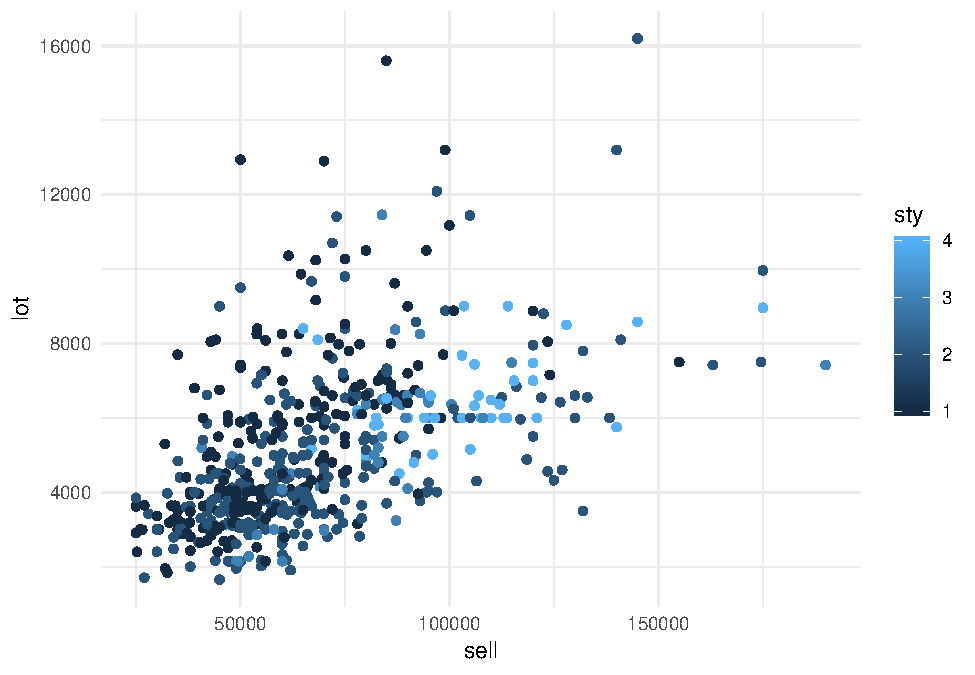
\includegraphics{Week6Assignment_files/figure-latex/unnamed-chunk-3-1.pdf}
The CPI logarithm log(CPI) plots indicate exactly the same things, and
the corresponding diagram looks very much similar to the previous one.

The apparently linear logarithmic increase confirms that the indexes
increase over time is probably logarithmic rather than linear.

\begin{Shaded}
\begin{Highlighting}[]
\NormalTok{g3\textless{}{-}}\StringTok{ }\KeywordTok{ggplot}\NormalTok{(}\KeywordTok{aes}\NormalTok{(}\DataTypeTok{x=} \KeywordTok{seq\_along}\NormalTok{(DPEUR), }\DataTypeTok{y=}\NormalTok{ DPEUR), }\DataTypeTok{data =}\NormalTok{ data)}\OperatorTok{+}\StringTok{ }\KeywordTok{geom\_line}\NormalTok{(}\DataTypeTok{color=} \StringTok{"red"}\NormalTok{)}\OperatorTok{+}
\StringTok{  }\KeywordTok{geom\_line}\NormalTok{(}\DataTypeTok{y=}\NormalTok{ data}\OperatorTok{$}\NormalTok{DPUSA, }\DataTypeTok{color=} \StringTok{"blue"}\NormalTok{) }\OperatorTok{+}
\StringTok{  }\KeywordTok{ggtitle}\NormalTok{(}\StringTok{"DPEUR(red) and DPUSA(blue) Evolution"}\NormalTok{)}

\KeywordTok{print}\NormalTok{(g3)}
\end{Highlighting}
\end{Shaded}

\begin{verbatim}
## Warning: Removed 1 rows containing missing values (geom_path).

## Warning: Removed 1 rows containing missing values (geom_path).
\end{verbatim}

\includegraphics{Week6Assignment_files/figure-latex/unnamed-chunk-4-1.pdf}

\hypertarget{b-perform-the-augmented-dickey-fuller-adf-test-for-the-two-logcpi-series.-in-the-adf-test-equation-include-a-constant-alpha-a-deterministic-trend-term-beta_t-three-lags-of-dp-deltalogcpi-and-of-course-the-variable-of-interest-logcpi_t-1.-report-the-coefficient-of-logcpi_t-1-and-its-standard-error-and-t-value-and-draw-your-conclusion.}{%
\paragraph{\texorpdfstring{(b) Perform the Augmented Dickey-Fuller (ADF)
test for the two log(CPI) series. In the ADF test equation, include a
constant (\(\alpha\)), a deterministic trend term (\(\beta_t\)), three
lags of DP = \(\Delta\)log(CPI) and, of course, the variable of interest
log(\(CPI_{t-1}\)). Report the coefficient of log(\(CPI_{t-1}\)) and its
standard error and t-value, and draw your
conclusion.}{(b) Perform the Augmented Dickey-Fuller (ADF) test for the two log(CPI) series. In the ADF test equation, include a constant (\textbackslash alpha), a deterministic trend term (\textbackslash beta\_t), three lags of DP = \textbackslash Deltalog(CPI) and, of course, the variable of interest log(CPI\_\{t-1\}). Report the coefficient of log(CPI\_\{t-1\}) and its standard error and t-value, and draw your conclusion.}}\label{b-perform-the-augmented-dickey-fuller-adf-test-for-the-two-logcpi-series.-in-the-adf-test-equation-include-a-constant-alpha-a-deterministic-trend-term-beta_t-three-lags-of-dp-deltalogcpi-and-of-course-the-variable-of-interest-logcpi_t-1.-report-the-coefficient-of-logcpi_t-1-and-its-standard-error-and-t-value-and-draw-your-conclusion.}}

\begin{Shaded}
\begin{Highlighting}[]
\NormalTok{adf1 \textless{}{-}}\StringTok{ }\KeywordTok{adf.test}\NormalTok{(data}\OperatorTok{$}\NormalTok{LOGPEUR,}\StringTok{\textquotesingle{}stationary\textquotesingle{}}\NormalTok{,}\DataTypeTok{k=}\DecValTok{3}\NormalTok{) }
\NormalTok{adf1}
\end{Highlighting}
\end{Shaded}

\begin{verbatim}
## 
##  Augmented Dickey-Fuller Test
## 
## data:  data$LOGPEUR
## Dickey-Fuller = -2.8263, Lag order = 3, p-value = 0.2324
## alternative hypothesis: stationary
\end{verbatim}

This adf.test always includes constant term and linear trend parameter.

\begin{Shaded}
\begin{Highlighting}[]
\NormalTok{adf1 \textless{}{-}}\StringTok{ }\KeywordTok{adf.test}\NormalTok{(data}\OperatorTok{$}\NormalTok{LOGPUSA,}\StringTok{\textquotesingle{}stationary\textquotesingle{}}\NormalTok{,}\DataTypeTok{k=}\DecValTok{3}\NormalTok{) }
\NormalTok{adf1}
\end{Highlighting}
\end{Shaded}

\begin{verbatim}
## 
##  Augmented Dickey-Fuller Test
## 
## data:  data$LOGPUSA
## Dickey-Fuller = -2.7345, Lag order = 3, p-value = 0.2706
## alternative hypothesis: stationary
\end{verbatim}

Both the series are not stationary! The ADF statistic is greater than
the critical value of −3.5.

\hypertarget{c-as-the-two-series-of-logcpi-are-not-cointegrated-you-need-not-check-this-we-continue-by-modelling-the-monthly-inflation-series-dpeurdeltalogcpieur-for-the-euro-area.-determine-the-sample-autocorrelations-and-the-sample-partial-autocorrelations-of-this-series-to-motivate-the-use-of-the-following-ar-model-dpeur_t-alpha-beta_1dpeur_t-6beta_2dpeur_t-12epsilon_t.-estimate-the-parameters-of-this-model-sample-jan-2000---dec-2010.}{%
\paragraph{\texorpdfstring{(c) As the two series of log(CPI) are not
cointegrated (you need not check this), we continue by modelling the
monthly inflation series DPEUR=\(\Delta\)log(CPIEUR) for the Euro area.
Determine the sample autocorrelations and the sample partial
autocorrelations of this series to motivate the use of the following AR
model:
\[DPEUR_t = \alpha + \beta_1DPEUR_{t-6}+\beta_2DPEUR_{t-12}+\epsilon_t\].
Estimate the parameters of this model (sample Jan 2000 - Dec
2010).}{(c) As the two series of log(CPI) are not cointegrated (you need not check this), we continue by modelling the monthly inflation series DPEUR=\textbackslash Deltalog(CPIEUR) for the Euro area. Determine the sample autocorrelations and the sample partial autocorrelations of this series to motivate the use of the following AR model: DPEUR\_t = \textbackslash alpha + \textbackslash beta\_1DPEUR\_\{t-6\}+\textbackslash beta\_2DPEUR\_\{t-12\}+\textbackslash epsilon\_t. Estimate the parameters of this model (sample Jan 2000 - Dec 2010).}}\label{c-as-the-two-series-of-logcpi-are-not-cointegrated-you-need-not-check-this-we-continue-by-modelling-the-monthly-inflation-series-dpeurdeltalogcpieur-for-the-euro-area.-determine-the-sample-autocorrelations-and-the-sample-partial-autocorrelations-of-this-series-to-motivate-the-use-of-the-following-ar-model-dpeur_t-alpha-beta_1dpeur_t-6beta_2dpeur_t-12epsilon_t.-estimate-the-parameters-of-this-model-sample-jan-2000---dec-2010.}}

First divide the data:

\begin{Shaded}
\begin{Highlighting}[]
\NormalTok{data\_orig\textless{}{-}}\StringTok{ }\KeywordTok{data.frame}\NormalTok{(data)}
\NormalTok{data[}\KeywordTok{which}\NormalTok{(data}\OperatorTok{$}\NormalTok{YYYY.MM }\OperatorTok{==}\StringTok{ "2010M12"}\NormalTok{), ]}
\end{Highlighting}
\end{Shaded}

\begin{verbatim}
##     YYYY.MM TREND CPI_EUR CPI_USA  LOGPEUR  LOGPUSA    DPEUR    DPUSA
## 132 2010M12   132   132.3   139.7 4.885072 4.939497 0.006065 0.001433
\end{verbatim}

\begin{Shaded}
\begin{Highlighting}[]
\NormalTok{data \textless{}{-}}\StringTok{ }\NormalTok{data[}\DecValTok{1}\OperatorTok{:}\DecValTok{132}\NormalTok{,]}
\NormalTok{f\_data \textless{}{-}}\StringTok{ }\NormalTok{data\_orig[}\DecValTok{133}\OperatorTok{:}\KeywordTok{nrow}\NormalTok{(data\_orig),]}
\end{Highlighting}
\end{Shaded}

\hypertarget{autocorrelations}{%
\paragraph{AutoCorrelations:}\label{autocorrelations}}

\begin{Shaded}
\begin{Highlighting}[]
\NormalTok{g1\textless{}{-}}\KeywordTok{ggAcf}\NormalTok{(data}\OperatorTok{$}\NormalTok{CPI\_EUR, }\DataTypeTok{type=}\StringTok{"correlation"}\NormalTok{)}
\NormalTok{g2\textless{}{-}}\KeywordTok{ggAcf}\NormalTok{(data}\OperatorTok{$}\NormalTok{CPI\_USA, }\DataTypeTok{type=}\StringTok{"correlation"}\NormalTok{)}
\NormalTok{g3\textless{}{-}}\KeywordTok{ggAcf}\NormalTok{(data}\OperatorTok{$}\NormalTok{LOGPEUR, }\DataTypeTok{type=}\StringTok{"correlation"}\NormalTok{)}
\NormalTok{g4\textless{}{-}}\KeywordTok{ggAcf}\NormalTok{(data}\OperatorTok{$}\NormalTok{LOGPUSA, }\DataTypeTok{type=}\StringTok{"correlation"}\NormalTok{)}
\NormalTok{g5\textless{}{-}}\KeywordTok{ggAcf}\NormalTok{(data}\OperatorTok{$}\NormalTok{DPEUR, }\DataTypeTok{type=}\StringTok{"correlation"}\NormalTok{)}
\NormalTok{g6\textless{}{-}}\KeywordTok{ggAcf}\NormalTok{(data}\OperatorTok{$}\NormalTok{DPUSA, }\DataTypeTok{type=}\StringTok{"correlation"}\NormalTok{)}
\KeywordTok{grid.arrange}\NormalTok{(g3,g4,g5,g6)}
\end{Highlighting}
\end{Shaded}

\includegraphics{Week6Assignment_files/figure-latex/unnamed-chunk-8-1.pdf}

\hypertarget{partial-autocorrelations}{%
\paragraph{Partial AutoCorrelations:}\label{partial-autocorrelations}}

\begin{Shaded}
\begin{Highlighting}[]
\NormalTok{g1\textless{}{-}}\KeywordTok{ggAcf}\NormalTok{(data}\OperatorTok{$}\NormalTok{CPI\_EUR, }\DataTypeTok{type=}\StringTok{"partial"}\NormalTok{)}
\NormalTok{g2\textless{}{-}}\KeywordTok{ggAcf}\NormalTok{(data}\OperatorTok{$}\NormalTok{CPI\_USA, }\DataTypeTok{type=}\StringTok{"partial"}\NormalTok{)}
\NormalTok{g3\textless{}{-}}\KeywordTok{ggAcf}\NormalTok{(data}\OperatorTok{$}\NormalTok{LOGPEUR, }\DataTypeTok{type=}\StringTok{"partial"}\NormalTok{)}
\NormalTok{g4\textless{}{-}}\KeywordTok{ggAcf}\NormalTok{(data}\OperatorTok{$}\NormalTok{LOGPUSA, }\DataTypeTok{type=}\StringTok{"partial"}\NormalTok{)}
\NormalTok{g5\textless{}{-}}\KeywordTok{ggAcf}\NormalTok{(data}\OperatorTok{$}\NormalTok{DPEUR, }\DataTypeTok{type=}\StringTok{"partial"}\NormalTok{)}
\NormalTok{g6\textless{}{-}}\KeywordTok{ggAcf}\NormalTok{(data}\OperatorTok{$}\NormalTok{DPUSA, }\DataTypeTok{type=}\StringTok{"partial"}\NormalTok{)}
\KeywordTok{grid.arrange}\NormalTok{(g3,g4,g5,g6)}
\end{Highlighting}
\end{Shaded}

\includegraphics{Week6Assignment_files/figure-latex/unnamed-chunk-9-1.pdf}

The lags with the largest values found from above gaps, are 6 and 12:

Thus, the findings motivate using lags 6 and 12 with the AR model. And
as this is not an MA model (residuals are not included), AR model could
be estimated using the OLS method (instead of the MLE method).

Estimating the AR model for lags 6 and 12 and using OLS, produces the
following Autoregressive Fit Model:

\begin{Shaded}
\begin{Highlighting}[]
\KeywordTok{library}\NormalTok{(dynlm)}
\end{Highlighting}
\end{Shaded}

\begin{verbatim}
## Warning: package 'dynlm' was built under R version 3.6.3
\end{verbatim}

\begin{Shaded}
\begin{Highlighting}[]
\NormalTok{ts\_logeur \textless{}{-}}\StringTok{ }\KeywordTok{ts}\NormalTok{(data}\OperatorTok{$}\NormalTok{DPEUR, }\DataTypeTok{start =}\DecValTok{2}\NormalTok{)}
\NormalTok{ar.model \textless{}{-}}\StringTok{ }\KeywordTok{dynlm}\NormalTok{(ts\_logeur }\OperatorTok{\textasciitilde{}}\StringTok{ }\KeywordTok{L}\NormalTok{(ts\_logeur, }\DecValTok{6}\NormalTok{) }\OperatorTok{+}\StringTok{ }\KeywordTok{L}\NormalTok{(ts\_logeur, }\DecValTok{12}\NormalTok{))}
\KeywordTok{summary}\NormalTok{(ar.model)}
\end{Highlighting}
\end{Shaded}

\begin{verbatim}
## 
## Time series regression with "ts" data:
## Start = 15, End = 133
## 
## Call:
## dynlm(formula = ts_logeur ~ L(ts_logeur, 6) + L(ts_logeur, 12))
## 
## Residuals:
##        Min         1Q     Median         3Q        Max 
## -0.0103343 -0.0017369 -0.0000475  0.0015322  0.0080903 
## 
## Coefficients:
##                   Estimate Std. Error t value Pr(>|t|)    
## (Intercept)      0.0003838  0.0002811   1.365   0.1749    
## L(ts_logeur, 6)  0.1887459  0.0772888   2.442   0.0161 *  
## L(ts_logeur, 12) 0.5979841  0.0835544   7.157 8.05e-11 ***
## ---
## Signif. codes:  0 '***' 0.001 '**' 0.01 '*' 0.05 '.' 0.1 ' ' 1
## 
## Residual standard error: 0.002569 on 116 degrees of freedom
##   (1 observation deleted due to missingness)
## Multiple R-squared:  0.4232, Adjusted R-squared:  0.4132 
## F-statistic: 42.55 on 2 and 116 DF,  p-value: 1.381e-14
\end{verbatim}

\hypertarget{d-extend-the-ar-model-of-part-c-by-adding-lagged-values-of-monthly-inflation-in-the-usa-at-lags-1-6-and-12.-check-that-the-coefficient-at-lag-6-is-not-significant-and-estimate-the-adl-model}{%
\paragraph{(d) Extend the AR model of part (c) by adding lagged values
of monthly inflation in the USA at lags 1, 6, and 12. Check that the
coefficient at lag 6 is not significant, and estimate the ADL
model}\label{d-extend-the-ar-model-of-part-c-by-adding-lagged-values-of-monthly-inflation-in-the-usa-at-lags-1-6-and-12.-check-that-the-coefficient-at-lag-6-is-not-significant-and-estimate-the-adl-model}}

\begin{Shaded}
\begin{Highlighting}[]
\NormalTok{train \textless{}{-}}\StringTok{ }\KeywordTok{ts.intersect}\NormalTok{(}\KeywordTok{ts}\NormalTok{(data}\OperatorTok{$}\NormalTok{DPEUR), }\KeywordTok{ts}\NormalTok{(data}\OperatorTok{$}\NormalTok{DPUSA))}
\KeywordTok{colnames}\NormalTok{(train) \textless{}{-}}\StringTok{ }\KeywordTok{c}\NormalTok{(}\StringTok{"dpEur"}\NormalTok{, }\StringTok{"dpUsa"}\NormalTok{)}
\NormalTok{model \textless{}{-}}\StringTok{ }\KeywordTok{dynlm}\NormalTok{(dpEur }\OperatorTok{\textasciitilde{}}\StringTok{ }\KeywordTok{L}\NormalTok{(dpEur, }\DecValTok{6}\NormalTok{) }\OperatorTok{+}\StringTok{ }\KeywordTok{L}\NormalTok{(dpEur, }\DecValTok{12}\NormalTok{) }\OperatorTok{+}\StringTok{ }\KeywordTok{L}\NormalTok{(dpUsa, }\DecValTok{1}\NormalTok{) }\OperatorTok{+}\StringTok{ }\KeywordTok{L}\NormalTok{(dpUsa, }\DecValTok{6}\NormalTok{) }\OperatorTok{+}\StringTok{ }\KeywordTok{L}\NormalTok{(dpUsa, }\DecValTok{12}\NormalTok{), }\DataTypeTok{data=}\NormalTok{train)}
\KeywordTok{summary}\NormalTok{(model)}
\end{Highlighting}
\end{Shaded}

\begin{verbatim}
## 
## Time series regression with "ts" data:
## Start = 14, End = 132
## 
## Call:
## dynlm(formula = dpEur ~ L(dpEur, 6) + L(dpEur, 12) + L(dpUsa, 
##     1) + L(dpUsa, 6) + L(dpUsa, 12), data = train)
## 
## Residuals:
##        Min         1Q     Median         3Q        Max 
## -0.0065866 -0.0016535 -0.0000118  0.0012630  0.0082682 
## 
## Coefficients:
##                Estimate Std. Error t value Pr(>|t|)    
## (Intercept)   0.0004407  0.0002853   1.545    0.125    
## L(dpEur, 6)   0.2029891  0.0785520   2.584    0.011 *  
## L(dpEur, 12)  0.6367464  0.0874766   7.279 4.78e-11 ***
## L(dpUsa, 1)   0.2264287  0.0511286   4.429 2.20e-05 ***
## L(dpUsa, 6)  -0.0560565  0.0547645  -1.024    0.308    
## L(dpUsa, 12) -0.2300418  0.0541695  -4.247 4.47e-05 ***
## ---
## Signif. codes:  0 '***' 0.001 '**' 0.01 '*' 0.05 '.' 0.1 ' ' 1
## 
## Residual standard error: 0.002272 on 113 degrees of freedom
##   (1 observation deleted due to missingness)
## Multiple R-squared:  0.5602, Adjusted R-squared:  0.5408 
## F-statistic: 28.79 on 5 and 113 DF,  p-value: < 2.2e-16
\end{verbatim}

The coefficient \(DPUSA_{t−6}\) is indeed not-significant.
(value=−0.056, t−statistic=−1.024, p−value=0.308).

\hypertarget{simplified-adl-model-estimation}{%
\subsubsection{Simplified ADL model
estimation}\label{simplified-adl-model-estimation}}

\begin{Shaded}
\begin{Highlighting}[]
\NormalTok{adl.model \textless{}{-}}\StringTok{ }\KeywordTok{dynlm}\NormalTok{(dpEur }\OperatorTok{\textasciitilde{}}\StringTok{ }\KeywordTok{L}\NormalTok{(dpEur, }\DecValTok{6}\NormalTok{) }\OperatorTok{+}\StringTok{ }\KeywordTok{L}\NormalTok{(dpEur, }\DecValTok{12}\NormalTok{) }\OperatorTok{+}\StringTok{ }\KeywordTok{L}\NormalTok{(dpUsa, }\DecValTok{1}\NormalTok{) }\OperatorTok{+}\StringTok{ }\KeywordTok{L}\NormalTok{(dpUsa, }\DecValTok{12}\NormalTok{), }\DataTypeTok{data=}\NormalTok{train)}
\KeywordTok{summary}\NormalTok{(adl.model)}
\end{Highlighting}
\end{Shaded}

\begin{verbatim}
## 
## Time series regression with "ts" data:
## Start = 14, End = 132
## 
## Call:
## dynlm(formula = dpEur ~ L(dpEur, 6) + L(dpEur, 12) + L(dpUsa, 
##     1) + L(dpUsa, 12), data = train)
## 
## Residuals:
##        Min         1Q     Median         3Q        Max 
## -0.0067809 -0.0016356  0.0000532  0.0013660  0.0082448 
## 
## Coefficients:
##                Estimate Std. Error t value Pr(>|t|)    
## (Intercept)   0.0003391  0.0002676   1.267   0.2076    
## L(dpEur, 6)   0.1687310  0.0710801   2.374   0.0193 *  
## L(dpEur, 12)  0.6551529  0.0856263   7.651 6.93e-12 ***
## L(dpUsa, 1)   0.2326460  0.0507772   4.582 1.19e-05 ***
## L(dpUsa, 12) -0.2264880  0.0540694  -4.189 5.55e-05 ***
## ---
## Signif. codes:  0 '***' 0.001 '**' 0.01 '*' 0.05 '.' 0.1 ' ' 1
## 
## Residual standard error: 0.002273 on 114 degrees of freedom
##   (1 observation deleted due to missingness)
## Multiple R-squared:  0.5561, Adjusted R-squared:  0.5406 
## F-statistic: 35.71 on 4 and 114 DF,  p-value: < 2.2e-16
\end{verbatim}

\hypertarget{e-use-the-models-of-parts-c-and-d-to-make-two-series-of-12-monthly-inflation-forecasts-for-2011.-at-each-month-you-should-use-the-data-that-are-then-available-for-example-to-forecast-inflation-for-september-2011-you-can-use-the-data-up-to-and-including-august-2011.-however-do-not-re-estimate-the-model-and-use-the-coefficients-as-obtained-in-parts-c-and-d.-for-each-of-the-two-forecast-series-compute-the-values-of-the-root-mean-squared-error-rmse-mean-absolute-error-mae-and-the-sum-of-the-forecast-errors-sum.-finally-give-your-interpretation-of-the-outcomes.}{%
\paragraph{(e) Use the models of parts (c) and (d) to make two series of
12 monthly inflation forecasts for 2011. At each month, you should use
the data that are then available, for example, to forecast inflation for
September 2011 you can use the data up to and including August 2011.
However, do not re-estimate the model and use the coefficients as
obtained in parts (c) and (d). For each of the two forecast series,
compute the values of the root mean squared error (RMSE), mean absolute
error (MAE), and the sum of the forecast errors (SUM). Finally, give
your interpretation of the
outcomes.}\label{e-use-the-models-of-parts-c-and-d-to-make-two-series-of-12-monthly-inflation-forecasts-for-2011.-at-each-month-you-should-use-the-data-that-are-then-available-for-example-to-forecast-inflation-for-september-2011-you-can-use-the-data-up-to-and-including-august-2011.-however-do-not-re-estimate-the-model-and-use-the-coefficients-as-obtained-in-parts-c-and-d.-for-each-of-the-two-forecast-series-compute-the-values-of-the-root-mean-squared-error-rmse-mean-absolute-error-mae-and-the-sum-of-the-forecast-errors-sum.-finally-give-your-interpretation-of-the-outcomes.}}

\hypertarget{adl-prediction}{%
\subsubsection{ADL Prediction}\label{adl-prediction}}

\begin{Shaded}
\begin{Highlighting}[]
\NormalTok{dpEur \textless{}{-}}\StringTok{ }\KeywordTok{ts}\NormalTok{(f\_data}\OperatorTok{$}\NormalTok{DPEUR)}
\NormalTok{dpUsa \textless{}{-}}\StringTok{ }\KeywordTok{ts}\NormalTok{(f\_data}\OperatorTok{$}\NormalTok{DPUSA)}
\NormalTok{test \textless{}{-}}\StringTok{ }\KeywordTok{ts.intersect}\NormalTok{(dpEur, dpUsa)}
\NormalTok{dependentvarname \textless{}{-}}\StringTok{ "dpEur"}
\NormalTok{x1\textless{}{-}}\StringTok{ "dpUsa"}

\NormalTok{Ntrain \textless{}{-}}\StringTok{ }\KeywordTok{nrow}\NormalTok{(train)}
\NormalTok{Ntest \textless{}{-}}\StringTok{ }\KeywordTok{nrow}\NormalTok{(test)}
\NormalTok{df\_train \textless{}{-}}\KeywordTok{data.frame}\NormalTok{(train)}
\NormalTok{df\_test \textless{}{-}}\StringTok{ }\KeywordTok{data.frame}\NormalTok{(test)}
\CommentTok{\# can\textquotesingle{}t rbind ts\textquotesingle{}s apparently, so convert to numeric first}
\NormalTok{df\_train[,dependentvarname] \textless{}{-}}\StringTok{ }\KeywordTok{as.numeric}\NormalTok{(df\_train[,dependentvarname])}
\NormalTok{df\_test[,dependentvarname] \textless{}{-}}\StringTok{ }\OtherTok{NA}
\NormalTok{df\_testtraindata \textless{}{-}}\StringTok{ }\KeywordTok{rbind}\NormalTok{( df\_train, df\_test )}
\NormalTok{df\_testtraindata[,dependentvarname] \textless{}{-}}\StringTok{ }\KeywordTok{ts}\NormalTok{( }\KeywordTok{as.numeric}\NormalTok{( df\_testtraindata[,dependentvarname] ) )}

\NormalTok{l1\textless{}{-}}\DecValTok{6}
\NormalTok{l2\textless{}{-}}\StringTok{ }\DecValTok{12}
\NormalTok{l3 \textless{}{-}}\StringTok{ }\DecValTok{1}
\NormalTok{l4 \textless{}{-}}\StringTok{ }\DecValTok{12}

\CommentTok{\# step through one by one}
\ControlFlowTok{for}\NormalTok{( i }\ControlFlowTok{in} \DecValTok{1}\OperatorTok{:}\NormalTok{Ntest ) \{}
\NormalTok{  result \textless{}{-}}\StringTok{ }\KeywordTok{sum}\NormalTok{(adl.model}\OperatorTok{$}\NormalTok{coeff }\OperatorTok{*}\StringTok{ }\KeywordTok{cbind}\NormalTok{(}\DecValTok{1}\NormalTok{, df\_testtraindata[Ntrain}\OperatorTok{+}\NormalTok{i}\OperatorTok{{-}}\NormalTok{l1, dependentvarname],}
\NormalTok{                                  df\_testtraindata[Ntrain}\OperatorTok{+}\NormalTok{i}\OperatorTok{{-}}\NormalTok{l2, dependentvarname],}
\NormalTok{                                  df\_testtraindata[Ntrain}\OperatorTok{+}\NormalTok{i}\OperatorTok{{-}}\NormalTok{l3, x1],}
\NormalTok{                                  df\_testtraindata[Ntrain}\OperatorTok{+}\NormalTok{i}\OperatorTok{{-}}\NormalTok{l4, x1]))}
\NormalTok{  df\_testtraindata[Ntrain}\OperatorTok{+}\NormalTok{i,dependentvarname] \textless{}{-}}\StringTok{ }\NormalTok{result}
  \KeywordTok{cat}\NormalTok{(}\StringTok{"predicted i"}\NormalTok{,i,}\StringTok{"of"}\NormalTok{,Ntest,}\StringTok{" :"}\NormalTok{,result,}\StringTok{"}\CharTok{\textbackslash{}n}\StringTok{"}\NormalTok{)}
\NormalTok{\}}
\end{Highlighting}
\end{Shaded}

\begin{verbatim}
## predicted i 1 of 12  : -0.00621878 
## predicted i 2 of 12  : 0.003634046 
## predicted i 3 of 12  : 0.008113709 
## predicted i 4 of 12  : 0.005836694 
## predicted i 5 of 12  : 0.002269904 
## predicted i 6 of 12  : 0.002658253 
## predicted i 7 of 12  : -0.003540649 
## predicted i 8 of 12  : 0.001792593 
## predicted i 9 of 12  : 0.004194302 
## predicted i 10 of 12  : 0.003641583 
## predicted i 11 of 12  : 0.0005755105 
## predicted i 12 of 12  : 0.004114096
\end{verbatim}

\begin{Shaded}
\begin{Highlighting}[]
\NormalTok{dpEur \textless{}{-}}\StringTok{ }\KeywordTok{ts}\NormalTok{(f\_data}\OperatorTok{$}\NormalTok{DPEUR)}
\NormalTok{dpUsa \textless{}{-}}\StringTok{ }\KeywordTok{ts}\NormalTok{(f\_data}\OperatorTok{$}\NormalTok{DPUSA)}
\NormalTok{test \textless{}{-}}\StringTok{ }\KeywordTok{ts.intersect}\NormalTok{(dpEur, dpUsa)}
\NormalTok{dependentvarname \textless{}{-}}\StringTok{ "dpEur"}

\NormalTok{Ntrain \textless{}{-}}\StringTok{ }\KeywordTok{nrow}\NormalTok{(train)}
\NormalTok{Ntest \textless{}{-}}\StringTok{ }\KeywordTok{nrow}\NormalTok{(test)}
\NormalTok{df\_train \textless{}{-}}\KeywordTok{data.frame}\NormalTok{(train)}
\NormalTok{df\_test \textless{}{-}}\StringTok{ }\KeywordTok{data.frame}\NormalTok{(test)}
\CommentTok{\# can\textquotesingle{}t rbind ts\textquotesingle{}s apparently, so convert to numeric first}
\NormalTok{df\_train[,dependentvarname] \textless{}{-}}\StringTok{ }\KeywordTok{as.numeric}\NormalTok{(df\_train[,dependentvarname])}
\NormalTok{df\_test[,dependentvarname] \textless{}{-}}\StringTok{ }\OtherTok{NA}
\NormalTok{ardf\_testtraindata \textless{}{-}}\StringTok{ }\KeywordTok{rbind}\NormalTok{( df\_train, df\_test )}
\NormalTok{ardf\_testtraindata[,dependentvarname] \textless{}{-}}\StringTok{ }\KeywordTok{ts}\NormalTok{( }\KeywordTok{as.numeric}\NormalTok{( ardf\_testtraindata[,dependentvarname] ) )}

\NormalTok{l1\textless{}{-}}\DecValTok{6}
\NormalTok{l2\textless{}{-}}\StringTok{ }\DecValTok{12}
\CommentTok{\#i=8}
\CommentTok{\# step through one by one}
\ControlFlowTok{for}\NormalTok{( i }\ControlFlowTok{in} \DecValTok{1}\OperatorTok{:}\NormalTok{Ntest ) \{}
\NormalTok{  result \textless{}{-}}\StringTok{ }\KeywordTok{sum}\NormalTok{(ar.model}\OperatorTok{$}\NormalTok{coeff }\OperatorTok{*}\StringTok{ }\KeywordTok{cbind}\NormalTok{(}\DecValTok{1}\NormalTok{, ardf\_testtraindata[Ntrain}\OperatorTok{+}\NormalTok{i}\OperatorTok{{-}}\NormalTok{l1, dependentvarname],}
\NormalTok{                                  ardf\_testtraindata[Ntrain}\OperatorTok{+}\NormalTok{i}\OperatorTok{{-}}\NormalTok{l2, dependentvarname]))}
\NormalTok{  ardf\_testtraindata[Ntrain}\OperatorTok{+}\NormalTok{i,dependentvarname] \textless{}{-}}\StringTok{ }\NormalTok{result}
  \KeywordTok{cat}\NormalTok{(}\StringTok{"predicted i"}\NormalTok{,i,}\StringTok{"of"}\NormalTok{,Ntest,}\StringTok{" :"}\NormalTok{,result,}\StringTok{"}\CharTok{\textbackslash{}n}\StringTok{"}\NormalTok{)}
\NormalTok{\}}
\end{Highlighting}
\end{Shaded}

\begin{verbatim}
## predicted i 1 of 12  : -0.00543937 
## predicted i 2 of 12  : 0.002532843 
## predicted i 3 of 12  : 0.007425756 
## predicted i 4 of 12  : 0.003708782 
## predicted i 5 of 12  : 0.0009842607 
## predicted i 6 of 12  : 0.001528509 
## predicted i 7 of 12  : -0.002931379 
## predicted i 8 of 12  : 0.001778539 
## predicted i 9 of 12  : 0.003613982 
## predicted i 10 of 12  : 0.002907036 
## predicted i 11 of 12  : 0.001024606 
## predicted i 12 of 12  : 0.004299039
\end{verbatim}

\begin{Shaded}
\begin{Highlighting}[]
\NormalTok{df\_testtraindata[}\DecValTok{130}\OperatorTok{:}\KeywordTok{nrow}\NormalTok{(df\_testtraindata),] }\OperatorTok{\%\textgreater{}\%}\StringTok{ }\KeywordTok{ggplot}\NormalTok{(}\KeywordTok{aes}\NormalTok{(}\DataTypeTok{x=}\KeywordTok{seq\_along}\NormalTok{(dpEur), }\DataTypeTok{y=}\NormalTok{dpEur,}\DataTypeTok{color=}\StringTok{"ADL Preiction"}\NormalTok{))}\OperatorTok{+}\KeywordTok{geom\_line}\NormalTok{()}\OperatorTok{+}
\StringTok{  }\KeywordTok{geom\_line}\NormalTok{(}\DataTypeTok{y=}\NormalTok{ data\_orig[}\DecValTok{130}\OperatorTok{:}\KeywordTok{nrow}\NormalTok{(data\_orig),]}\OperatorTok{$}\NormalTok{DPEUR, }\KeywordTok{aes}\NormalTok{(}\DataTypeTok{color=} \StringTok{"Original Data"}\NormalTok{))}\OperatorTok{+}\KeywordTok{ylim}\NormalTok{(}\OperatorTok{{-}}\FloatTok{0.01}\NormalTok{, }\FloatTok{0.02}\NormalTok{)}\OperatorTok{+}
\KeywordTok{geom\_line}\NormalTok{(}\DataTypeTok{y=}\NormalTok{ ardf\_testtraindata[}\DecValTok{130}\OperatorTok{:}\KeywordTok{nrow}\NormalTok{(ardf\_testtraindata),]}\OperatorTok{$}\NormalTok{dpEur, }\KeywordTok{aes}\NormalTok{(}\DataTypeTok{color=} \StringTok{"AR Prediction"}\NormalTok{))}
\end{Highlighting}
\end{Shaded}

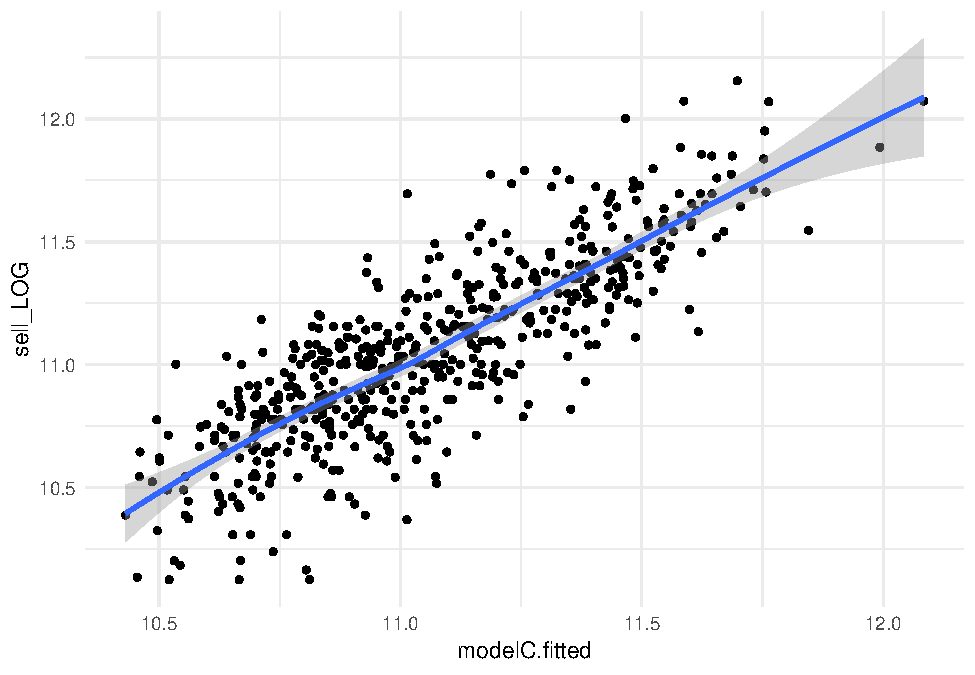
\includegraphics{Week6Assignment_files/figure-latex/unnamed-chunk-15-1.pdf}

\begin{Shaded}
\begin{Highlighting}[]
\NormalTok{RMSE =}\StringTok{ }\ControlFlowTok{function}\NormalTok{(m, o)\{}
  \KeywordTok{sqrt}\NormalTok{(}\KeywordTok{mean}\NormalTok{((m }\OperatorTok{{-}}\StringTok{ }\NormalTok{o)}\OperatorTok{\^{}}\DecValTok{2}\NormalTok{))}
\NormalTok{\}}
\KeywordTok{cat}\NormalTok{(}\StringTok{"RMSE For ADL: "}\NormalTok{,}\KeywordTok{RMSE}\NormalTok{(df\_testtraindata[}\DecValTok{133}\OperatorTok{:}\KeywordTok{nrow}\NormalTok{(df\_testtraindata),]}\OperatorTok{$}\NormalTok{dpEur,data\_orig[}\DecValTok{133}\OperatorTok{:}\KeywordTok{nrow}\NormalTok{(data\_orig),]}\OperatorTok{$}\NormalTok{DPEUR), }\StringTok{"}\CharTok{\textbackslash{}n}\StringTok{"}\NormalTok{)}
\end{Highlighting}
\end{Shaded}

\begin{verbatim}
## RMSE For ADL:  0.002216519
\end{verbatim}

\begin{Shaded}
\begin{Highlighting}[]
\KeywordTok{cat}\NormalTok{(}\StringTok{"RMSE For AR: "}\NormalTok{,}\KeywordTok{RMSE}\NormalTok{(ardf\_testtraindata[}\DecValTok{133}\OperatorTok{:}\KeywordTok{nrow}\NormalTok{(ardf\_testtraindata),]}\OperatorTok{$}\NormalTok{dpEur,data\_orig[}\DecValTok{133}\OperatorTok{:}\KeywordTok{nrow}\NormalTok{(data\_orig),]}\OperatorTok{$}\NormalTok{DPEUR), }\StringTok{"}\CharTok{\textbackslash{}n}\StringTok{"}\NormalTok{)}
\end{Highlighting}
\end{Shaded}

\begin{verbatim}
## RMSE For AR:  0.002491731
\end{verbatim}

\begin{Shaded}
\begin{Highlighting}[]
\NormalTok{MAE =}\StringTok{ }\ControlFlowTok{function}\NormalTok{(m, o)\{}
  \KeywordTok{mean}\NormalTok{(}\KeywordTok{abs}\NormalTok{(m}\OperatorTok{{-}}\NormalTok{o))}
\NormalTok{\}}
\KeywordTok{cat}\NormalTok{(}\StringTok{"MAE For ADL: "}\NormalTok{,}\KeywordTok{MAE}\NormalTok{(df\_testtraindata[}\DecValTok{133}\OperatorTok{:}\KeywordTok{nrow}\NormalTok{(df\_testtraindata),]}\OperatorTok{$}\NormalTok{dpEur,data\_orig[}\DecValTok{133}\OperatorTok{:}\KeywordTok{nrow}\NormalTok{(data\_orig),]}\OperatorTok{$}\NormalTok{DPEUR), }\StringTok{"}\CharTok{\textbackslash{}n}\StringTok{"}\NormalTok{)}
\end{Highlighting}
\end{Shaded}

\begin{verbatim}
## MAE For ADL:  0.001490881
\end{verbatim}

\begin{Shaded}
\begin{Highlighting}[]
\KeywordTok{cat}\NormalTok{(}\StringTok{"MAE For AR: "}\NormalTok{,}\KeywordTok{MAE}\NormalTok{(ardf\_testtraindata[}\DecValTok{133}\OperatorTok{:}\KeywordTok{nrow}\NormalTok{(ardf\_testtraindata),]}\OperatorTok{$}\NormalTok{dpEur,data\_orig[}\DecValTok{133}\OperatorTok{:}\KeywordTok{nrow}\NormalTok{(data\_orig),]}\OperatorTok{$}\NormalTok{DPEUR), }\StringTok{"}\CharTok{\textbackslash{}n}\StringTok{"}\NormalTok{)}
\end{Highlighting}
\end{Shaded}

\begin{verbatim}
## MAE For AR:  0.0018659
\end{verbatim}

\begin{Shaded}
\begin{Highlighting}[]
\NormalTok{SUM =}\StringTok{ }\ControlFlowTok{function}\NormalTok{(m, o)\{}
  \KeywordTok{sum}\NormalTok{(}\KeywordTok{abs}\NormalTok{(m }\OperatorTok{{-}}\StringTok{ }\NormalTok{o))}
\NormalTok{\}}
\KeywordTok{cat}\NormalTok{(}\StringTok{"SUM For ADL: "}\NormalTok{,}\KeywordTok{SUM}\NormalTok{(df\_testtraindata[}\DecValTok{133}\OperatorTok{:}\KeywordTok{nrow}\NormalTok{(df\_testtraindata),]}\OperatorTok{$}\NormalTok{dpEur,data\_orig[}\DecValTok{133}\OperatorTok{:}\KeywordTok{nrow}\NormalTok{(data\_orig),]}\OperatorTok{$}\NormalTok{DPEUR), }\StringTok{"}\CharTok{\textbackslash{}n}\StringTok{"}\NormalTok{)}
\end{Highlighting}
\end{Shaded}

\begin{verbatim}
## SUM For ADL:  0.01789057
\end{verbatim}

\begin{Shaded}
\begin{Highlighting}[]
\KeywordTok{cat}\NormalTok{(}\StringTok{"SUM For AR: "}\NormalTok{,}\KeywordTok{SUM}\NormalTok{(ardf\_testtraindata[}\DecValTok{133}\OperatorTok{:}\KeywordTok{nrow}\NormalTok{(ardf\_testtraindata),]}\OperatorTok{$}\NormalTok{dpEur,data\_orig[}\DecValTok{133}\OperatorTok{:}\KeywordTok{nrow}\NormalTok{(data\_orig),]}\OperatorTok{$}\NormalTok{DPEUR), }\StringTok{"}\CharTok{\textbackslash{}n}\StringTok{"}\NormalTok{)}
\end{Highlighting}
\end{Shaded}

\begin{verbatim}
## SUM For AR:  0.0223908
\end{verbatim}

\hypertarget{conclusion}{%
\subsubsection{Conclusion:}\label{conclusion}}

Clearly, the ADL model performed better forecasts than the AR model, as
it scored less at all errors scores.

This means that the insight used in part (d), about using the USA
monthly inflation series at lags 1 and 12 in order to forecast the EURO
monthly inflation, was correct.


\end{document}
